%% Author - Matthew A Robson
\documentclass{beamer}
\usepackage{tikz}
\usepackage{quantikz}
\usepackage{textcomp}
\usepackage{amsmath}
\usepackage{hyperref}
\usepackage{physics}
\usepackage{graphicx}
\usetikzlibrary{positioning, angles, quotes}

\usetheme{Berkeley}
\usecolortheme{default}

%% I want to fix a few color and theme things to match my school
\definecolor{MySchoolBlue}{RGB}{0, 51, 102}
\setbeamercolor{structure}{fg=MySchoolBlue, bg=MySchoolBlue}
\setbeamercolor{item}{fg=MySchoolBlue}
\setbeamercolor{enumerate item}{fg=MySchoolBlue}
\setbeamercolor{itemize item}{fg=MySchoolBlue}


\title[Quantum Computing] %% includes the title on every slides
{High Speed Computing with Clustered and Quantum Computers}
\subtitle{}
\author[Robson, Matthew] %% includes my name on every slide
{M.~A.~Robson\inst{1}}

\institute[VFU] %% include the institution and further specifying information
{
  %\inst{1}%
  LASA{CS} Department\\
  Liberal Arts and Science Academy
  \and
  %\inst{2}%
  Period 1\\
  Independent Study Computer Science
}

\date[VLC 2021] %% include the date and even of the presentation
{Fall Final, December 2025}

\logo{\begin{tikzpicture}
% \filldraw[color=red!50, fill=red!25, very thick](0,0) circle (0.5);
% \node[draw,color=white] at (0,0) {LOGO HERE};
\node (myImage) at (0,0) {\includegraphics[width=0.15\textwidth]{logo.png}};
\end{tikzpicture}}

%End of title page configuration block
%------------------------------------------------------------
%The next block of commands puts the table of contents at the 
%beginning of each section and highlights the current section:

\AtBeginSection[]
{
  \begin{frame}
    \frametitle{Table of Contents}
    \tableofcontents[currentsection]
  \end{frame}
}
%------------------------------------------------------------
\begin{document}


%%%% Page 1 -- Title Page
\frame{\titlepage}

%%%% Page 2 -- Introduction 
\begin{frame}
\frametitle{What Is Quantum Computing?}

Quantum computing covers many concepts, but it is important to first start with classical computing.

\begin{block}{Classical Information}
In a classical computer it stores information as a 1 or a 0 in what is called a bit.
\end{block}

\begin{exampleblock}{Some Common Gates}
NAND, NOR, AND, OR, XOR $\rightarrow$ Complex structures such as ALUs and data storage.  
\end{exampleblock}

\begin{quantikz}
  \lstick{A} & \gate{NOT} & \rstick{$\bar{A}$}
\end{quantikz}

\end{frame}

%%%% Page 3 -- Time Complexity and Circuit Complexity
\begin{frame}
\frametitle{Circuit Complexity}

In circuits it is important to cover the complexity required to achieve certain goals.
Complexity is classified in Big O Notation.
\newline
\newline
Additionally, we can classify these further into P, NP, NP-complete, etc.

\begin{exampleblock}{Time Complexity Example}
  A loop of N elements has a time complexity of $\mathcal{O}(N)$.
\end{exampleblock}

\begin{alertblock}{Theorem 1.0}
  Any NP complete problem can be solve in polynomial time on a classical computer.
\end{alertblock}

\end{frame}

%%%% Page 4 -- Final Classical Computing 

\begin{frame}
\frametitle{Turing Completeness}

Simply, a Turing-complete computer is one that is able to compute any and Turing-computable function.

\begin{block}{Definition 1.0}
  Some computational device is taken as Turing-complete or Turing-equivalent if it is probable that it can compute the values for a function for every function of its argument.\ ie. A common place computer.
\end{block}

While Turing-complete computers are powerful, they begin to break down at the meta level in cases such as the infamous Halting Problem.\ (see the LASACS lunch time lecture)

\end{frame}

%%%% Page 5 -- Introduction to Quantum Computers and Qubits

\begin{frame}
\frametitle{A Single Qubit}



\centering %% Include the bloch sphere that I created for my notes
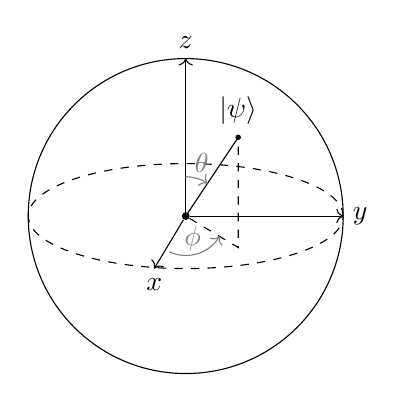
\begin{tikzpicture}

  % Define radius
  \def\r{2}

  % Bloch vector
  \draw (0,0) node[circle, fill, inner sep=1] (orig) {} -- (\r/3,\r/2)
    node[circle, fill, inner sep=0.7, label=above:$\ket{\psi}$] (a) {};
  \draw[dashed] (orig) -- (\r/3, -\r/5) node (phi) {} -- (a);

  % Sphere
  \draw (orig) circle (\r);
  \draw[dashed] (orig) ellipse (\r{} and \r/3);

  % Axes
  \draw[->] (orig) -- ++(-\r/5, -\r/3) node[below] (x1) {$x$};
  \draw[->] (orig) -- ++(\r, 0) node[right] (x2) {$y$};
  \draw[->] (orig) -- ++(0, \r) node[above] (x3) {$z$};

  % Angles
  \pic [draw=gray, text=gray, ->, "$\phi$"] {angle = x1--orig--phi};
  \pic [draw=gray, text=gray, <-, "$\theta$", angle eccentricity=1.4] {angle = a--orig--x3};

\end{tikzpicture}

\end{frame}



\end{document}